\documentclass[14pt]{article}

\usepackage[utf8x]{inputenc}
\usepackage[russian]{babel}
\usepackage{graphicx}
\usepackage{bm}
\usepackage{amssymb,amsmath}
\usepackage[export]{adjustbox}
\usepackage{subcaption}
\usepackage{float}
\usepackage{wrapfig}
\graphicspath{{images/}}
\DeclareGraphicsExtensions{.pdf,.png,.jpg}

\usepackage{amsmath}
\usepackage{pgfplots}

\usepackage{geometry} % Меняем поля страницы
\geometry{left=2cm}% левое поле
\geometry{right=1.5cm}% правое поле
\geometry{top=2cm}% верхнее поле
\geometry{bottom=2cm}% нижнее поле

\begin{document}
\begin{titlepage}
	\begin{center}
		\vspace*{6cm}
		\fontsize{24pt}{25pt}\selectfont
		Поляризация света при рассеянии.
		
		Оптическая активность.
	\end{center}
	\begin{flushright}
		\fontsize{18pt}{20pt}\selectfont
		\vspace{12cm}
		\hspace{-3cm}
		\textit{Корнеев Е.С.\\Группа 713}
	\end{flushright}		
\end{titlepage}

\begin{center}
	\fontsize{16pt}{18pt}\selectfont
	Поляризация света при рассеянии.
		
	Оптическая активность.
\end{center}

\fontsize{14pt}{16pt}\selectfont
Данная работа представляет из себя две практически независимые части, связанные с поляризацией света при рассении и с оптической активностью веществ.

\section{Поляризация света при рассеянии}

1. В прозрачной однородной среде бегущая плоская волна распространяется только в прямом направении, не испытывая рассеяния в стороны (будем считать, что ширина фронта волны достаточно велика, чтобы пренебречь явлением дифракционной расходимости). Допустим, что оптическая однородность среды нарушена, например, множеством мельчайших частиц постороннего вещества, беспорядочно распределенных по объему среды. Примерами могут служить пыльный воздух, туман, дым, эмульсии. Тогда показатель преломления будет меняться в пространстве весьма нерегулярно, но среднее значение его во всяком малом объеме, содержащем еще очень много макроскопических неоднородностей, будет оставаться одним и тем же во всей среде. Такую среду называют \textsl{оптически мутной}. В оптически мутных средах свет распространяется не только в прямом направлении, но и рассеивается в стороны. Рассеяние света в мутных средах на частицах постороннего вешества экспериментально впервые исследовал Тиндаль (1820-1893) в 1869~г. Поэтому это явление получило название \textsl{тиндалевского рассеяния} или \textsl{эффекта Тиндаля}. Его теория была дана Рэлеем.

2. В неоднородной неподвижной изотропной среде распространение света описывается уравнениями Максвелла
\begin{equation}
\begin{aligned}
	\operatorname{rot}\vec{H} = \frac{\varepsilon}{c}\frac{\partial\vec E}{\partial t},~~~\operatorname{div}(\varepsilon\vec{E}) = 0,\\
	\operatorname{rot}\vec{E} = -\frac{1}{c}\frac{\partial\vec H}{\partial t},~~~\operatorname{div}\vec{H} = 0,
\end{aligned}
\end{equation}
где диэлектрическая проницаемость $\varepsilon$ является функцией координат. Выделим из нее постоянную часть $\varepsilon_0$, полагая
$\varepsilon = \varepsilon_0 + \delta\varepsilon$. В проблеме рассеяния света интерес представляет случай, когда $\delta\varepsilon$ мало по сравнению с $\varepsilon_0$, но пока мы не будем вводить этого ограничения. Более того, постоянное слагаемое $\varepsilon_0$ в принципе можно было бы выбрать произвольно. От этого, если вычисления производить точно, окончательный результат зависеть не может. Однако удобно и естественно понимать под $\varepsilon_0$ диэлектрическую проницаемость среды, из которой удалены частицы постороннего вещества.

Представим электромагнитное поле в виде $\vec{E} = \vec{E_0} + \vec{E'}$, $\vec{H} = \vec{H_0} + \vec{H'}$, где $E_0$, $H_0$ удовлетворяют уравнениям Максвелла в однородной среде
$$
\begin{aligned}
	\operatorname{rot}\vec{H_0} = \frac{\varepsilon_0}{c}\frac{\partial\vec E_0}{\partial t},~~~\operatorname{div}(\varepsilon\vec{E_0}) = 0,\\
	\operatorname{rot}\vec{E_0} = -\frac{1}{c}\frac{\partial\vec H_0}{\partial t},~~~\operatorname{div}\vec{H_0} = 0.
\end{aligned}
$$

В задаче о рассеянии света это есть падающая волна, которая распространялась бы в среде, если бы в ней не было оптических неоднородностей, а $\vec{E'}$, $\vec{H'}$ -- поле рассеянного света. Вычитая предыдущие уравнения из (1), получим
\begin{equation}
\begin{aligned}
	\operatorname{rot}\vec{H'} - \frac{\varepsilon_0}{c}\frac{\partial\vec E'}{\partial t} = \frac{\delta\varepsilon}{c}\frac{\partial\vec E'}{\partial t},~~~
	\operatorname{div}(\varepsilon_0\vec{E'}) = -\operatorname{div}(\delta\varepsilon\vec{E}),	\\
	\operatorname{rot}\vec{E'} - \frac{1}{c}\frac{\partial\vec H'}{\partial t},~~~~~~~~~~~~~~~~~~~~~~~~~~~~~~~~~~~\operatorname{div}\vec{H'} = 0.
\end{aligned}
\end{equation}

Таким образом, для поля $\vec{E'}$, $\vec{H'}$ получились такие же уравнения Максвелла, как в однородной среде с диэлектрической проницаемостью $\varepsilon_0$. Только первые два из этих уравнений содержат правые части, которые можно рассматривать как дополнительные источники электромагнитных волн. Если ввести обозначение
\begin{equation}
	\delta\vec{P} = \frac{\delta\varepsilon}{4\pi}\vec{E}
\end{equation}
то эти два уравнения перейдут в
\begin{equation}
	\operatorname{rot}\vec{H'} - \frac{\varepsilon_0}{c}\frac{\partial\vec E'}{\partial t} = \frac{4\pi}{c}\frac{\partial}{\partial t}\vec{\delta\vec{P}},~~~
	\operatorname{div}(\varepsilon_0\vec{E'}) = -4\pi\operatorname{div}(\delta\varepsilon\vec{E})
\end{equation}
Из них видно, что в среде появляется дополнительная поляризация $\delta P$, определяемая выражением (3), так что каждый малый элемент объема среды $\delta V$ получает дополнительный дипольный момент $\delta V\cdot\delta P$. Меняясь во времени, он излучает электромагнитные волны как колеблющийся диполь Герца. Это и есть свет, рассеянный элементом объема $\delta V$.

3. Допустим теперь, что оптическая неоднородность создается одинаковыми шариками радиуса $a$, беспорядочно распределенными по объему, занятому средой. Пусть среднее расстояние между шариками велико по сравнению с $a$, а сами шарики малы по сравнению с длиной волны. Тогда при вычислении электрического поля $\vec{E}$ внутри шарика можно считать внешнее поле $\vec{E_0}$ световой волны однородным. Как показано в электростатике, поле $\vec{E}$ также однородно и определяется выражением
\begin{equation}
	\vec{E} = \frac{3}{\varepsilon/\varepsilon_0 + 2}\vec{E_0} = \frac{3\varepsilon_0}{\varepsilon + 2\varepsilon_0}\vec{E_0},
\end{equation}
где $\varepsilon$ -- диэлектрическая проницаемость шарика, а $\varepsilon_0$ -- окружающей среды. Дополнительная поляризация, согласно формуле (3), будет отлична от нуля только внутри шариков, где она равна
$$
	\delta\vec{P} = \frac{\varepsilon-\varepsilon_0}{4\pi}\vec{E} = \frac{\varepsilon-\varepsilon_0}{4\pi}\frac{3\varepsilon_0}{\varepsilon + 2\varepsilon_0}\vec{E_0}
$$
а дополнительный дипольный момент шарика
\begin{equation}
	\vec{p} = \frac{\varepsilon_0}{\varepsilon + 2\varepsilon_0}(\varepsilon - \varepsilon_0)a^3\vec{E_0}.
\end{equation}

Предположим сначала, что падающая волна поляризована линейно. Тогда векторы $\vec{p}$ и $\vec{E}$ все время будут параллельны одному и тому же неизменному направлению. Электрическое поле диполя $\vec{p}$ на больших расстояниях $r$ от него (в волновой зоне) определяется выражением
\begin{equation}
	E_1 = -\frac{\omega^2\sin\varphi}{c^2r}p_{t-r/v}
\end{equation}
где $v = c/\sqrt{\varepsilon} = c/n$ - скорость света в рассматриваемой среде, $\varphi$ - угол между осью диполя $\vec{p}$ и направлением рассеянного излучения.  Рассеянный свет поляризован линейно, причем электрический вектор лежит в плоскости, проходящей через ось диполя $\vec{p}$ и направление излучения. Под интенсивностью света здесь и в дальнейшем будем понимать усредненное по времени численное значение вектора Пойнтинга. Для интенсивности света, рассеянного одним шариком, электродинамика дает
\begin{equation}
	I_1 = \frac{\omega^4\sin^2\varphi}{4\pi\varepsilon_0v^3r^2}\overline{p^2}.
\end{equation}
Интенсивность прямой волны равна
\begin{equation}
	I_0 = \frac{c}{4\pi}\overline{E_0H_0} = \frac{v}{4\pi}\varepsilon_0\overline{E_0^2}
\end{equation}

Воспользовавшись (6), получим
\begin{equation}
	I_1 = 9\varepsilon_0^2\left(\frac{\varepsilon - \varepsilon_0}{\varepsilon + 2\varepsilon_0}\right)\frac{\omega^2a^6\sin^2\varphi}{c^4r^2}I_0
\end{equation}
или
\begin{equation}
	I_1 = 9\varepsilon_0^2\left(\frac{\varepsilon - \varepsilon_0}{\varepsilon + 2\varepsilon_0}\right)\frac{\pi^2V_1^2}{\lambda^4}\frac{\sin^2\varphi}{r^2}I_0
\end{equation}

где $\lambda$ -- длина волны в вакууме, а $V_1 = \frac{4}{3}\pi a^3$ -- объем шарика. Энергия $P_1$, рассеиваемая шариком в единицу времени по всем направлениям, найдется интегрированием величины (11) по сфере радиуса $r$. Взяв в качестве элемента поверхности $2\pi r^2\sin\varphi d\theta$, получим
\begin{equation}
	P_1 = 24\pi^3\varepsilon_0^2\left(\frac{\varepsilon - \varepsilon_0}{\varepsilon + 2\varepsilon_0}\right)\frac{V_1^2}{\lambda^4}I_0
\end{equation}

Допустим теперь, что падающий свет естественный. Направление его распространения примем за ось $Z$. Пусть рассеянный свет наблюдается в направлении $OA$ под углом $\theta$ оси $Z$. Угол $\theta$ называется углом рассеяния (рис. 1). Направим ось $X$ перпендикулярно к $OA$ и $OZ$. Так как $\vec{p}$ и $\vec{E_0}$ коллинеарны, то вектор $\vec{p}$ параллелен плоскости $XY$. Разложим его по осям $X$ и $Y$. Интенсивности излучений дипольных моментов $\vec{p_x}$ и $\vec{p_y}$ найдутся по формуле (8), если в ней положить сначала $\varphi = \pi/2$, а затем $\varphi = \pi/2 - \theta$ Так как падающий свет естественный, то эти излучения некогерентины, так что для нахождения $I_1$ надо сложить их интенсивности. В результате формула (8) перейдет в
$$
	I_1 =   \frac{\omega^4}{4\pi\varepsilon_0v^3r^2}(\overline{p_x^2} + \overline{p_y^2}\cos\theta) = 
			\frac{\omega^4}{4\pi\varepsilon_0v^3r^2}\frac{1+\cos^2\theta}{2}\overline{p^2},
$$
так как в случае естественного света, $\overline{p_x^2} = \overline{p_y^2} = 1/2\overline{p^2}$. Следовательно, вместо формулы (11) получится
\begin{equation}
	I_1 = 9\varepsilon_0^2\left(\frac{\varepsilon - \varepsilon_0}{\varepsilon + 2\varepsilon_0}\right)\frac{\pi^2V_1^2}{\lambda^4}\frac{1+\cos^2\theta}{2r^2}I_0
\end{equation}
Формула (12), очевидно, останется без изменения.

\begin{wrapfigure}{R}{7cm}
\centering
	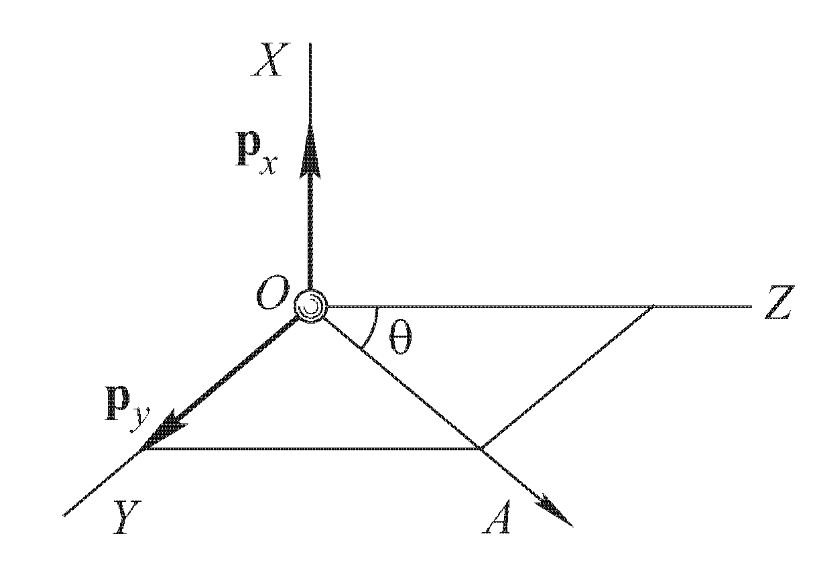
\includegraphics[width=7cm]{1.png}
	\caption{К выводу зависимости интенсивности от угла}
\end{wrapfigure}

Теперь рассеянный свет будет поляризован частично. Полная линейная поляризация будет наблюдаться только в тех случаях, когда линия наблюдения $OA$ перпендикулярна к направлению распространения падающего света, так как в этом случае дипольный момент $\vec{p_y}$ излучения не дает. 

Найдем теперь интенсивность $I$ света, рассеиваемого объемом $V$, содержащим очень много шариков. Их среднее число в этом объеме равно $NV$, где $N$ -- среднее число шариков
в единице объема. Так как расстояния между шариками велики по сравнению с $a$ и они распределены по объему $V$ беспорядочно, то для нахождения $I$ надо сложить интенсивности, рассеиваемые отдельными шариками. Предположим, что расстояние от объема $V$ до точки наблюдения велико по сравнению с линейными размерами самого объема $V$. Тогда в формуле (13) все расстояния $r$ можно считать одинаковыми и написать
\begin{equation}
	I = 9\varepsilon_0^2\left(\frac{\varepsilon - \varepsilon_0}{\varepsilon + 2\varepsilon_0}\right)\frac{\pi^2V_1^2}{\lambda^4}\frac{1+\cos^2\theta}{2r^2}NVI_0
\end{equation}

4. Для наблюдения эффекта используем пробирку, наполненную смесью воды и молока. Сверху установим фонарик белого света и поляризатор. Используя поляризатор, нетрудно определить плоскость поляризации света. Действительно, на фотографиях видно, что есть направление поляризатора, при котором столб света виден заметно ярче, чем при другом положении, то есть действительно можно наблюдать эффект Тиндаля. При этом рассеяние во все стороны происходит с одинаковой интенсивностью, чего и стоило ожидать.

\begin{figure}[h!]
	\center{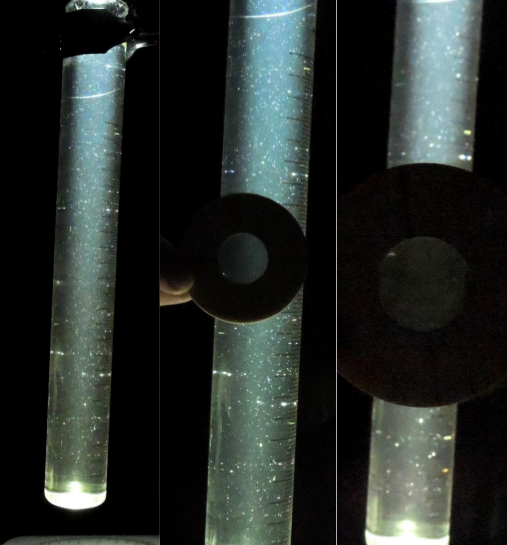
\includegraphics[height=15cm]{Milk_2}} 
	\caption{Рассеяние света}
\end{figure}

\newpage

\setcounter{equation}{0}
\setcounter{figure}{0}

\section{Оптическая активность}

1. Если линейно поляризованный свет проходит через плоскопараллельный слой вещества, то в некоторых случаях плоскость поляризации света оказывается повернутой относительно
своего исходного положения. Это явление называется \textsl{вращением плоскости поляризации} или \textsl{оптической активностью}. Если вещество не находится во внешнем магнитном поле, то оптическая активность и вращение плоскости поляризации называются \textsl{естественными}. В противоположном случае говорят о \textsl{магнитном вращении плоскости поляризации} или \textsl{эффекте Фарадея}.

Естественная активность была открыта в 1811 г. Араго на пластинках кварца, вырезанных перпендикулярно к оптической оси. В 1815 г. Био подробно исследовал это явление, а также обнаруженное им вращение плоскости поляризации в растворах сахара. Затем естественное вращение плоскости поляризации было найдено у многих других тел. К концу прошлого века число известных естественно-активных веществ превышало 700. Теперь их известно гораздо больше, хотя для большинства вешеств, где обнаружено это явление, оно выражено очень слабо.

Для наблюдения явления можно установить на оптической скамье два скрещенных николя. Такая система не пропускает свет. Однако, если между николями ввести пластинку кварца, вырезанную перпендикулярно к оптической оси, или слой какого-либо другого оптически активного вещества, то свет через систему будет проходить. Но его можно погасить вращением одного из николей. Отсюда следует, что после прохождения через активное ветцество свет остается линейно поляризованным, но его плоскость поляризации оказывается повернутой. Для успеха, опыта падающий свет, если он белый, необходимо монохроматизировать, пропустив его через светофильтр, так как \textsl{угол поворота плоскости поляризации зависит от длины волны}. Кварц -- одноосный кристалл. В описанном опыте свет распространяется вдоль оптической оси, когда кварц ведет себя как изотропное тело, не давая обычного (линейного) двойного лучепреломления.

В зависимости от взятого вещества естественное вращение плоскости поляризации может происходить вправо или влево, причем эти два направления условились относить к наблюдателю, к которому свет приближается. В соответствии с этим различают \textsl{право-} и \textsl{левовращающие вещества}. Вращение вправо считается \textsl{положительным}, а влево -- \textsl{отрицательным}.

2. Явление вращения плоскости поляризации указывает на определенную дисимметрию, свойственную оптически активным средам. Она выражается в том, что в таких средах направления вращения по и против часовой стрелки физически не эквивалентны. Поэтому в среде не может быть плоскости симметрии, проходящей через направление нормали к фронту волны. Иначе, как это следует из общих соображений симметрии, плоскость поляризации света не могла бы врашаться, если бы она совпадала с любой из плоскостей симметрии. В то же время естественно-активные среды, если они жидкие, полностью изотропны, т.е. все направления в них совершенно эквивалентны. Это проявляется, в частности, в том, что естественно-активная жидкость вращает плоскость поляризации в одну и ту же сторону, независимо от направления распространения света. Поэтому естественно-активную жидкость можно охарактеризовать как дисимметрично-изотропную среду. В кристаллах нет изотропии, но в одноосных кристаллах всякие два взаимно противоположные направления оптической оси также эквивалентны, по крайней мере в оптическом отношении.

Отмеченная дисимметрия напоминает дисимметрию винтовой спирали. Будем смотреть на один из торцов спирали. Пусть по спирали движется точка, вращаясь по часовой стрелке. Если
при этом точка удаляется от нас, то спираль называется правой (в противоположном случае она называется левой). Если посмотреть на спираль с противоположного торца, то вращение той же точки будет происходить против часовой стрелки, но в этом случае точка будет приближаться к нам. Чтобы она удалялась, надо направление вращения изменить на противоположное. Таким образом, свойство спирали быть правой или левой не зависит от того, с какого торца на нее смотреть. Так и свойство естественно-активной среды быть право- или левовращающей не зависит от того, в каком из двух прямо противоположных направлений распространяется свет.

Таким образом, если плоскость поляризации в естественноактивной среде врашается, например, вправо, то при изменении направления распространения света на противоположное
она по-прежнему будет вращаться вправо. Однако направления вращения <<вправо>> и <<влево>> относятся к разным наблюдателям: к каждому из них свет должен приближаться. Объективно, независимо от выбора наблюдателя, вращения происходят в противоположные стороны, если лучи распространяются навстречу друг другу. Если свет заставить пройти туда
и обратно через естественно-активное вещество, отразив его от зеркала, то плоскость поляризации возвратится к своему исходному направлению.

3. Кварц встречается в природе в виде двух модификаций: правовращающего и левовращающего (короче -- правого и левого). Это явление называется \textsl{энантиоморфизмом} и встречается у кристаллов, не содержащих центров и плоскостей симметрии. Обе энантиоморфные модификации кристалла отличаются друг от друга внешней формой и внутренней кристаллической
структурой. По своей симметрии они отличаются друг от друга примерно так же, как правая спираль отличается от левой или правая рука от левой. Таким образом, обе модификации не \textsl{конгруэнтны}, т.е. правая не может быть наложена на левую и наоборот. Но зеркальное изображение одной из этих модификаций может быть совмещено с другой. Поидимому, все естественно-активные кристаллы существуют в двух энантиоморфных модификациях, хотя не во всех случаях известны обе модификации. Некоторые жидкости, например винная кислота, могут встречаться также в виде двух модификаций, вращающих плоскость поляризации в противоположных направлениях.

4. Био установил на опыте, что угол поворота $\varphi$ плоскости поляризации пропорционален толщине $l$ оптически активного вещества: $\varphi = \alpha l$, где коэффициент 
$\alpha$ называется вращением на единицу длины. Он зависит от длины волны, природы вещества и температуры. Для кварца при температуре 20 $^\circ$С и желтого света натрия 
($\lambda = 589,3$ нм) $\alpha = \pm21,728$, для хлорноватистокислого натрия ($NaClO_3$) $\alpha = 3,170$ угловых градуса на миллиметр. Для некоторых жидких кристаллов 
$\alpha$ может достигать 40000 градусов на миллиметр. Для правых и левых модификаций кварца, и всех остальных кристаллов значения вращения $\alpha$ о\textsl{динаковы по величине, но противоположны по знаку}. Вращение $\alpha$ увеличивается с уменьшением длины волны. Био нашел, что величина $\alpha$ обратно пропорциональна квадрату длины волны 
$\lambda$. Но такая зависимость грубо приближенна. В области прозрачности и малого поглощения хорошо согласуется с опытом формула Друде
$$
	\alpha = \sum_i \frac{B_i}{\lambda^2 - \lambda_i^2},
$$
где $B_i$ -- постоянные, $\lambda_i$ -- длины волн, cоответствующие собственным частотам рассматриваемого вещества. 

5. Первое объяснение вращения плоскости поляризации было предложено Френелем в 1817 г. Его идея состояла в том, что для волн с различной круговой поляризацией (рис. 1) скорость распространения различна.

\begin{figure}[h!]

\begin{subfigure}{0.5\textwidth}
	\centering
	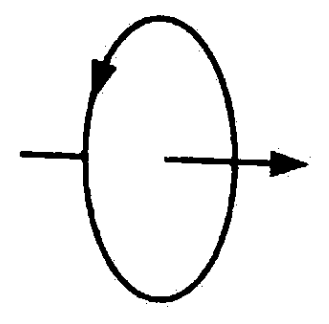
\includegraphics[height=4cm]{Left} 
	\caption{Левая}
\end{subfigure}
\begin{subfigure}{0.5\textwidth}
	\centering
	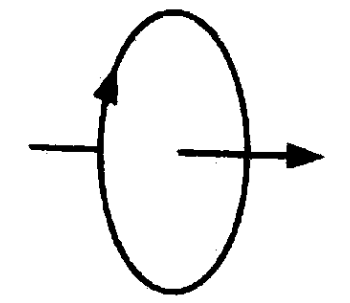
\includegraphics[height=4cm]{Right}
	\caption{Правая}
\end{subfigure}
	\caption{Круговые поляризации волн}
	
\end{figure}

Запишем волны с круговой поляризацией. Пусть волны распространяются вдоль оси $z$ и им отвечают волновые векторы $k_r$ и $k_l$ (соответственно для правой и левой поляризаций). Тогда для правой поляризации имеем
\begin{equation}
	E_x^r = E_0\cos(\omega t - k_rz),~~~E_y^r = E_0\cos(\omega t - k_rz + \pi/2)
\end{equation}
и для левой --
\begin{equation}
	E_x^l = E_0\cos(\omega t - k_lz),~~~E_y^l = E_0\cos(\omega t - k_lz - \pi/2)
\end{equation}
Обозначая
\begin{equation}
	k_r = k + \alpha,~~~k_l = k - \alpha,
\end{equation}
запишем суперпозицию волн (1) и (2):
\begin{equation}
\begin{aligned}
	E_x = E_x^r + E_x^l = 2E_0\cos(\alpha z)\cos(\omega t - kz)	\\
	E_y = E_y^r + E_y^l = 2E_0\sin(\alpha z)\cos(\omega t - kz).
\end{aligned}
\end{equation}

Очевидно, что в каждом сечении $z$ это линейно поляризованная волна. Однако её плоскость поляризации на пути $l$ поворачивается на угол
\begin{equation}
	\varphi = \alpha l.
\end{equation}

Свяжем угол вращения с показателями преломления для соответствующих волн. По определению фазовой скорости на основании (3) имеем
\begin{equation}
	v_r = \frac{\omega}{k_r} = \frac{\omega}{k + \alpha},~~~v_l = \frac{\omega}{k_l} = \frac{\omega}{k - \alpha}
\end{equation}
С другой стороны, фазовая скорость связана с показателем преломдения соотношением $v = c/n$, так что
\begin{equation}
	n_r = \frac{c}{v_r} = \frac{c}{\omega}(k + \alpha),~~~n_l = \frac{c}{v_l} = \frac{c}{\omega}(k - \alpha).
\end{equation}
Следовательно,
\begin{equation}
	n_r - n_l = \frac{2c}{\omega}\alpha
\end{equation}
или
\begin{equation}
	\alpha = \frac{\omega}{2c}(n_r - n_l) = \frac{\pi}{\lambda}(n_r - n_l).
\end{equation}

В соответствии с приведенным выше определением при $\alpha < 0$ мы имеем дело с положительным вращением, а при $\alpha > 0$ -- с отрицательным.

6. Приведенное рассуждение отнюдь не доказывает, что каждая из поляризованных по кругу волн (1) и (2) может в отдельности существовать в среде. Мы исходили из опытного факта, что в оптически активной среде может реально существовать волна с вращающейся плоскостью поляризации. Такая волна, конечно, должна быть решением системы фундаментальных уравнений Максвелла, дополненной материальными уравнениями в оптически активной среде. Должна удовлетворять этой системе уравнений и суперпозиция поляризованных по кругу волн (1) и (2), так как мы доказали, что такая суперпозиция дает волну с вращающейся плоскостью поляризации. Но любое решение всякой системы уравнений можно представить (и притом бесконечным числом способов) в виде суммы нескольких слагаемых, которые вовсе не обязательно должны быть решениями той же системы. Поэтому из того факта, что в оптически активной среде возможна волна с вращающейся плоскостью поляризации, еще не следует, что в ней возможны и одиночные волны с круговой поляризацией. Однако Френель предположил, что поляризованные по кругу волны со скоростями (6) действительно могут распространяться в оптически активной среде.

Их можно назвать \textsl{нормальными волнами}, т.е. такими волнами, которые распространяются в среде с сохранением своей формы и характера поляризации. Это предположение есть гипотеза, которую теоретически Френель доказать не мог, так как для этого необходимо было бы располагать полной системой уравнений волновой теории света в оптически активных средах. Но Френель подтвердил свою гипотезу экспериментально.

\begin{wrapfigure}{L}{10cm}
\centering
	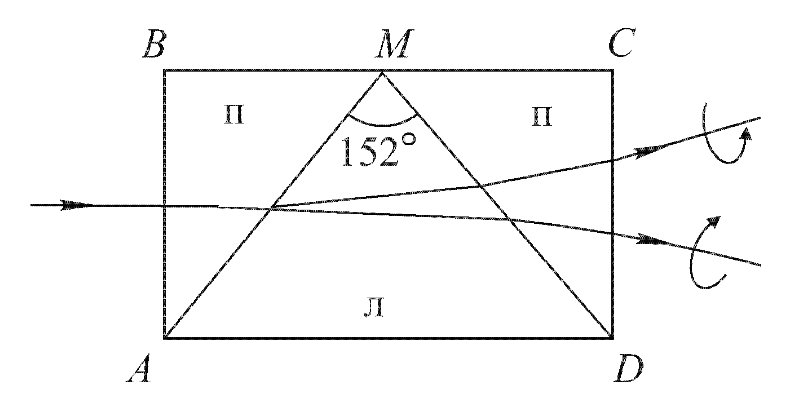
\includegraphics[width=10cm]{2}
	\caption{Опыт Френеля}
\end{wrapfigure}

Френель изготовил сложную призму, состоящую из трех кварцевых призм: двух призм $ABM$ и $DCM$ из правовращаюшего кварца и одной $AMD$ из левоврашающего с тупым углом 
$M = 152^\circ$ (рис. 2). Оптические оси всех трех призм были параллельны основанию $AD$. Падающий луч, параллельный оптической оси, на грани $AB$ не испытывал преломления, но разлагался внутри призмы $ABM$ на два луча, поляризованные по кругу. Луч с правой поляризацией, как показывают формулы (7), имел меньший, а луч с левой поляризацией -- больший показатель преломления ($n_r > n_l$). В левовращающей призме $AMD$ соотношение между этими показателями преломлени было обратным ($n_r < n_l$). Поэтому на грани $AM$ лучи испытывали разное преломление: правый луч приближался к основанию $AD$, а левый удалялся. Угол расхождения между лучами еще больше увеличивался при преломлении на гранях $DM$ и $CD$. В результате из призмы выходили лва луча: один отклонялся вниз, а другой вверх, угол расхождения между которыми составлял около 4’. Исследование при помощи пластинки $\lambda/4$ показало, что луч, отклонившийся вниз, был поляризован по правому, а вверх -- по левому кругу.

Френель предлагал проверить свою гипотезу и для жидкостей путем комбинации большого ряда призм, попеременно наполненных жидкостями, вращающими плоскость поляризации вправо и влево. Позднее такой опыт был осуществлен и показал, что и в оптически активных жидкостях также могут существовать две волны с различной круговой поляризацией: правой и левой.

Таким образом, Френель доказал экспериментально, что при вступлении в оптически активную среду луч света испытывает двойное круговое лучепреломление: лучи, поляризованные по
правому и левому кругу, идут внутри отптически активной среды с различными фазовыми скоростями. Если падающий свет был поляризован линейно, то при выходе из такой среды эти волны складываются снова в линейно поляризованную волну, но с повернутой плоскостью поляризации. Тем самым задача объяснения врашения плоскости поляризации была сведена к задаче объяснения кругового двойного лучепреломления.

7. Пронаблюдаем явление на опыте. Используем ту же установку, что и в предыдущем эксперименте, но теперь расположим второй поляризатор под пробиркой. Вращая его, будем добиваться максимально возможного затемнения луча. В пробирку нальем раствор фруктозы и будем понемногу удалять шприцом часть раствора. Тогда нам не важно, насколько была повернута поляризация после прохождения всего столба жидкости, а также то, что поляризатор повернут на 90 градусов по отношению к поляризации волны -- над достаточно лишь знать угол относительно начального положения поляризатора. Также в силу постоянства сечения пробирки удобнее снимать зависимость $\varphi(V)$, а не $\varphi(h)$. Величины 
$V$ и $h$ связаны соотношением
$$
	h/V = (0.91 \pm 0.02) \text{мм/мл}
$$
что нетрудно получить, сняв зависимость высоты жидкости от налитого в пробирку объема. В силу очевидной простоты измерений и отсутствия существенной связи с экспериментом, опустим подробное изложение метода и сами измерения.

Приведем результаты измерений положения поляризатора, при которых достигалась минимальная яркость луча при его прохождении через раствор:

\begin{center}
\begin{tabular}{|c|c|c|c|c|c|c|c|c|c|c|c|}
\hline
\multicolumn{4}{|c|}{Красный лазер}	&	\multicolumn{4}{|c|}{Красный лазер}	\\
\hline
$V$, мл	&	$\Delta V$, мм	&	$\varphi, ^\circ$	&	$\Delta\varphi, ^\circ$	&	$V$, мл	&	$\Delta V$, мм	&	$\varphi, ^\circ$	&	$\Delta\varphi, ^\circ$		\\
\hline
250		&	2				&	0					&	5						&	300		&	2				&	0					&	5							\\
\hline
230		&	2				&	20					&	5						&	250		&	2				&	55					&	5							\\
\hline
210		&	2				&	30					&	5						&	200		&	2				&	100					&	5							\\
\hline
190		&	2				&	45					&	5						&	150		&	2				&	145					&	5							\\
\hline
170		&	2				&	55					&	5						&	100		&	2				&	185					&	5							\\
\hline
150		&	2				&	65					&	5						&	50		&	2				&	230					&	5							\\
\hline
100		&	2				&	90					&	5						&	30		&	2				&	250					&	5							\\
\hline
50		&	2				&	120					&	5						&			&					&						&								\\
\hline
20		&	2				&	140					&	5						&			&					&						&								\\
\hline
\end{tabular}
\end{center}

Погрешность угла определим, вращая поляризатор. Так как точно сказать, когда разрешенное направление поляризатора ортогонально с поляризацией волны, сложно, будем оценивать эту величину, слегка вращая поляирзатор в окрестности минимума. В какой-то момент будет заметно, что интенсивность станет увеличиваться, этот угол и примем равным погрешности. 

Построим графики:

\begin{flushleft}
\begin{tikzpicture}
\begin{axis}[
	height = 8cm,
	width  = 15cm,
	every axis y label/.style={at = {(ticklabel cs: 0.5)}, rotate = 90, anchor = near ticklabel},
	xlabel = {$V$, мл},
	ylabel = {$\varphi, ^\circ$},
	xtick  = {0,50,100,150,200,250,300},
	ytick  = {0,50,100,150,200,250,300},
%	y tick label style={/pgf/number format/fixed zerofill}
]
\addplot+[%error bars/.cd, 
	%y dir = both, y explicit,
	%x dir = both, x explicit,
	only marks
	]
coordinates{
	(250, 0)	+- (2,5)
	(230, 20)	+- (2,5)
	(210, 30)	+- (2,5)
	(190, 45)	+- (2,5)
	(170, 55)	+- (2,5)
	(150, 65)	+- (2,5)
	(100, 90)	+- (2,5)
	( 50, 120)	+- (2,5)
	( 20, 140)	+- (2,5)
};
\addplot [mark = none]
coordinates{
	(250, 6.31545)
	(20, 139.13)
};



\addplot+[%error bars/.cd, 
	%y dir = both, y explicit,
	%x dir = both, x explicit,
	only marks
	]
coordinates{
	(300, 0)	+- (2,5)
	(250, 55)	+- (2,5)
	(200, 100)	+- (2,5)
	(150, 145)	+- (2,5)
	(100, 185)	+- (2,5)
	( 50, 230)	+- (2,5)
	( 30, 250)	+- (2,5)
};
\addplot [mark = none]
coordinates{
	(300, 6.02683)
	(30, 250.301)
};

\end{axis}
\end{tikzpicture}
\end{flushleft}

Из полученных графиков видно, что угол поворота плоскости поляризации излучения в растворе фруктозы является линейной функцией глубины проникновения света в раствор. Угловые коэффициенты линейной аппроксимации определим по МНК:
$$
	\frac{d\varphi}{dV} = -0.58 \frac{\text{град}}{\text{мл}},
$$
$$
	\frac{d\varphi}{dV} = -0.90 \frac{\text{град}}{\text{мл}}
$$
для красного и зеленого лазеров соответственно. Погрешности определим, считая $\sigma = \sqrt{\sigma_\text{приб}^2 + \sigma_\text{случ}^2}$, причем $\sigma_\text{случ}$ определим по МНК, а $\sigma_\text{приб}$ -- считая $d\varphi/dV = f(\varphi, V)$. Отсюда:
$$
	\frac{d\varphi}{dV} = (-0.58 \pm 0.05) \frac{\text{град}}{\text{мл}},
$$
$$
	\frac{d\varphi}{dV} = (-0.90 \pm 0.08) \frac{\text{град}}{\text{мл}}
$$
или же, приводя к привычному виду:
$$
	\frac{d\varphi}{dh} = (0.53 \pm 0.05)  \frac{\text{град}}{\text{мм}},
$$
$$
	\frac{d\varphi}{dh} = (0.82 \pm 0.08)  \frac{\text{град}}{\text{мм}}
$$

Также интересно будет изучить зависимость угла поворота от концентрации фруктозы. Для этого будем удалять часть раствора и доливать такое же количество воды. Так как начальную концентрацию мы не знаем, будем измерять отношение концентрации к начальному ее значению. Измерения проведем только для красного лазера. Таким образом:

\begin{center}
\begin{tabular}{|c|c|c|c|c|c|c|c|c|c|}
\hline
$\Delta V$, мм	&	$N$		&	$\varphi, ^\circ$	&	$\Delta\varphi, ^\circ$		\\
\hline
0				&	1.00	&	65					&	5							\\
\hline
20				&	0.87	&	77					&	5							\\
\hline
25				&	0.72	&	88					&	5							\\
\hline
50				&	0.48	&	112					&	5							\\
\hline
70				&	0.26	&	130					&	5							\\
\hline
100				&	0.09	&	141					&	5							\\
\hline
\end{tabular}
\end{center}

\begin{flushleft}
\begin{tikzpicture}
\begin{axis}[
	height = 9cm,
	width  = 15cm,
	every axis y label/.style={at = {(ticklabel cs: 0.5)}, rotate = 90, anchor = near ticklabel},
	xlabel = {$N$},
	ylabel = {$\varphi, ^\circ$},
	xtick  = {0,0.2,0.4,0.6,0.8,1.0},
	ytick  = {50,75,100,125,150},
%	y tick label style={/pgf/number format/fixed zerofill}
]
\addplot+[%error bars/.cd, 
	%y dir = both, y explicit,
	%x dir = both, x explicit,
	only marks
	]
coordinates{
	(   1, 65)	+- (0,5)
	(0.87, 77)	+- (0,5)
	(0.72, 88)	+- (0,5)
	(0.48, 112)	+- (0,5)
	(0.26, 130)	+- (0,5)
	(0.09, 141)	+- (0,5)
};
\addplot [mark = none]
coordinates{
	(1, 65.5554)
	(0.09, 143.035)
};

\end{axis}
\end{tikzpicture}
\end{flushleft}

Видно, что полученная зависимость также является линейной. Из двух полученных зависимостей можно сделать вывод, что зависимость можно описать формулой
$$	
	\varphi = \beta\cdot Nl
$$
где $\beta$ - некоторая константа, зависящая от длины волны. 

\newpage
Объединяя эффекты поляризации света при рассеянии и оптическую активность вещества, можно пронаблюдать вращение плоскости поляризации.

\begin{figure}[h!]

\begin{subfigure}{0.5\textwidth}
	\center{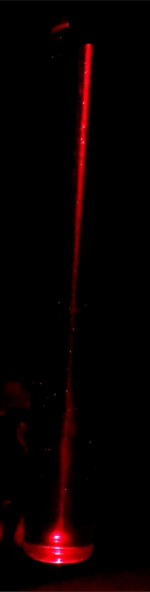
\includegraphics[height=20cm]{RedTwist_2}} 
	\caption{Вращение плоскости поляризации красного лазера}
\end{subfigure}
\begin{subfigure}{0.5\textwidth}
	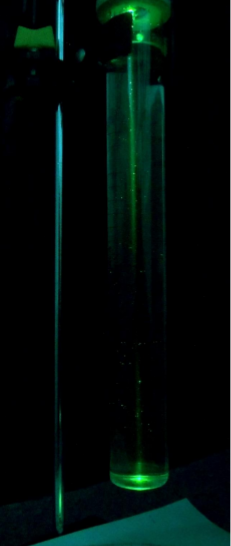
\includegraphics[height=20cm]{GreenTwist_2} 
	\caption{Вращение плоскости поляризации зеленого лазера}
\end{subfigure}

\end{figure}

Также используем фонарик белого света вместо лазера. Мы уже знаем, что для различных длин волн скорости поворота плоскостей поляризации отличается. Это самое интересное -- при наличии рассеяния мы можем наблюдать <<радугу>> в пробирке. Появление цветной спирали объясняется тем, что на какой-то глубине может реализоваться ситуация, что, скажем, красная составляющая спектра будет поляризована в плоскости, перпендикулярной плоскости наблюдения, а плоскость поляризации зеленой составляющей будет совпадать с плоскостью наблюдения. В итоге из белого света будет <<вырезан>> зеленый цвет, а красный будет преобладать.

\begin{figure}[h!]
	\center{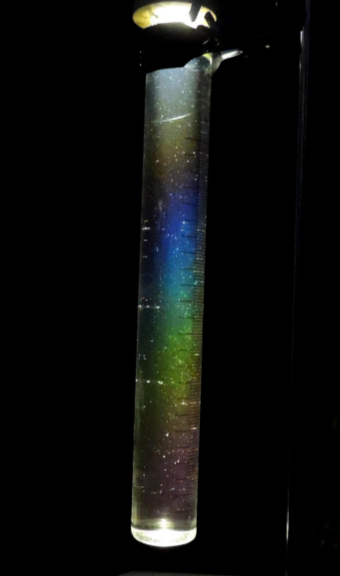
\includegraphics[height=20cm]{Rainbow_2}} 
	\caption{<<Радуга>> в колбе}
\end{figure}

\newpage
При подготовке данного вопроса по выбору использовавиль источники:

\begin{enumerate}
\item Сивухин Д.В. Общий курс физики. Оптика, 4-е издание.
\item Сивухин Д.В. Общий курс физики. Электричество, 6-е издание.
\item Кириченко Н.А. Принципы оптики.
\item Кизель В.А. Физические принципы диссимметрии живых систем.
\end{enumerate}



\end{document}

